\documentclass{beamer}


\usepackage[utf8]{inputenc}
 
 


%% Language and font encodings
\usepackage[english]{babel}



%% Useful packages
\usepackage{amsmath}
\usepackage{graphicx}
\usepackage[colorinlistoftodos]{todonotes}
\usepackage[colorlinks=true, allcolors=blue]{hyperref}
\usepackage{amssymb}
\usepackage[english]{babel}
\usepackage{amsthm}
\usepackage{multirow,array}
\usepackage{booktabs}
\usepackage{caption, threeparttable}
\usepackage{setspace}
\usepackage{blindtext}
\usepackage{breakcites}
\usepackage{blindtext,pdflscape}
\usepackage{rotating}
\usepackage{float}
\usepackage{multirow}
\usepackage{lscape}
\usepackage{xcolor}
\usepackage{mathtools}



%%plotting
\usepackage{tikz}
\usepackage{pgfplots}
\pgfplotsset{compat=1.14}
\usepgfplotslibrary{fillbetween}
\usetikzlibrary{patterns}

%custom
\newcommand{\bb}[1]{\mathbb{#1}}
\newcommand{\pderiv}[2]{ \frac{\partial#1}{\partial#2} }
\newcommand{\E}{\mathbb{E}}
\newcommand{\V}{\mathbb{V}}
\newcommand{\C}{\mathbb{C}ov}
\newcommand{\Lagr}{\mathcal{L}} %lagrangian
\let\biconditional\leftrightarrow


%Information to be included in the title page:
\title{Does Reality Match?: Empirical retrospectives of UPP \& HHI theories by Garmon (2017) }
\author{presented by Alex Kaufman}
\institute{WWS Legal and Regulatory Policy}
\date{3/5/2019}



\begin{document}
\frame{\titlepage}
 
\begin{frame}
\frametitle{Overview}
\begin{enumerate}
    \item Hospital Mergers
    \item Data sources
    \item Theory
    \item Estimation
    \item Results
    \item Limitations

\end{enumerate}
\end{frame}


\begin{frame}{Intro: Hospital Mergers}

    \begin{enumerate}
        \item Number of hospital mergers between 1997-2001 where FTC lost every case and prices went up a lot.
        \item Useful because we can evaluate predictive power of merger analysis methods without selection bias caused by blocked mergers.
        \item Hospital mergers have a big impact on the economy!
        \item tools used from class include HHI, Diversion Ratios, UPP.
    \end{enumerate}
\end{frame}

\begin{frame}{The Data}
            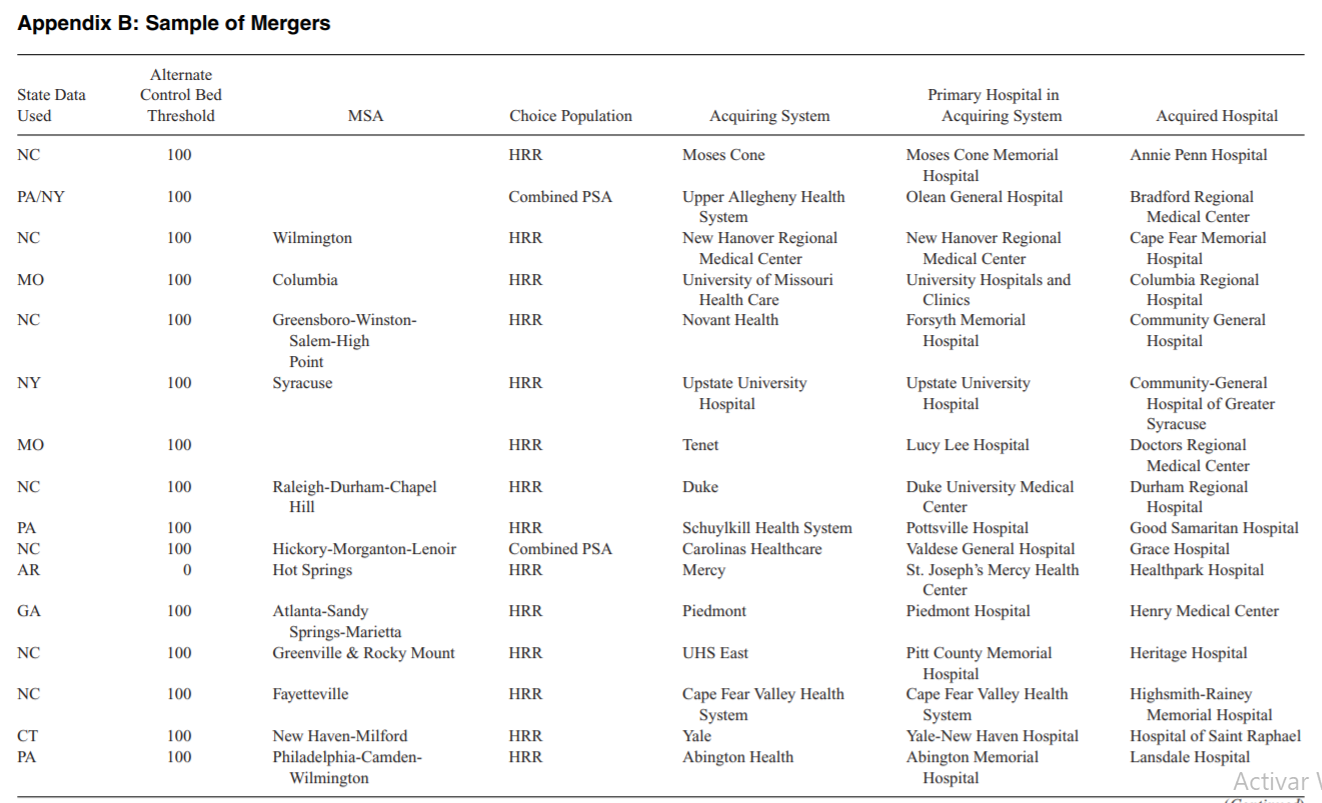
\includegraphics[width=\linewidth,height=\textheight,keepaspectratio]{data.PNG} \\
            N = 12
\end{frame}

\begin{frame}{UPP model}
MCO k, \\
New customers who join because of coverage at hospital j - $y_j$ \\
New people admitted to hospital j because of coverage - $y_h$ \\
People admitted to alternative hospital i - $y_i$
\begin{align*}
\pi_k & = Premium \times policy - costs \times policy\  - payment\ \times admit (h) \\
    & = \rho_{k} y_{j} - c_ky_{j} - \sum p_{j} y_{h} 
\end{align*}

\begin{align*}
\max_{p_j} \{ ( \underbrace{ \rho_{k}y_{j} - c_ky_{j} - p_jy_{h}}_{\text{k's profit from adding j}})^{(1-\gamma)}( \underbrace{ p_{j}y_{h}-c_{j}y_{h})^{\gamma} }_{\text{j's new proft}} \}
\end{align*}
\begin{equation*}
\text{FOCs give:    }        P_j = \frac{\gamma \pi_k+(1-\gamma)c_jy_{h}}{y_{h}} 
\end{equation*}
\end{frame}
\begin{frame}

\begin{align*}
    \max_{p_j} \{ ( \underbrace{ \rho_{k}y_{j} - c_ky_{j} - p_jy_{h}}_{\text{k's profit from including j}})^{(1-\gamma)}( \underbrace{ p_{j}y_{h}-c_{j}y_{h} - d_{hi}( \overbrace{p_{j}y_{i}-c_{j}y_{i} }^{\text{ diverted profit}})^{\gamma} }_{\text{j's net profit }} \}
\end{align*}
\begin{align*}
\text{FOCs give:    }        P_j & = \frac{\gamma \pi_k+(1-\gamma)c_jy_{h}} {y_{h}} + (1-\gamma)(p_i - c_i)d_{hi} \\
\end{align*}
$$
\%\Delta p_j = \frac{p^{post} - p_j}{p_j} = (1-\gamma)\bigg( \frac{p_i-c_i}{p_i} \bigg) \bigg( \frac{p_i}{p_j} \bigg) d_{hi}
$$
\end{frame}
\begin{frame}{HHI}
for market m \\
\\
$$HHI_m = \sum_{h \in m} s_h^2$$

where m is the area in which $<$ 10\% of people leave the area for service and where $<$ 10\% of patients are from outside the area.\\

and $s_h$ is 
\begin{itemize}
    \item the share of beds
    \item the share of admissions of patients residing in the area
\end{itemize}

\end{frame}
\begin{frame}{Estimation}

Estimate prices 
$$
\bar{P}_{ht} = \alpha_t P_{ht} + \epsilon_{ht},\ \ \ \ \epsilon \sim N(0,\sigma)
$$


Estimate price changes
$$
P_{ht} = \alpha + \beta_1 POST_{ht} + \beta_2 POST_{ht}\times MERGED_{ht} + \Gamma \delta_h + \epsilon_{ht}
$$


\end{frame}
\begin{frame}{Results}
            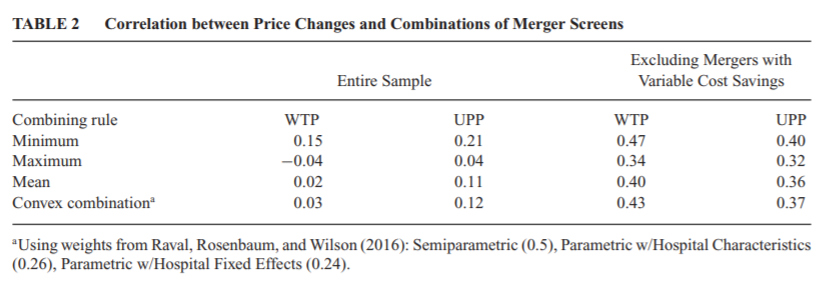
\includegraphics[width=\linewidth,height=\textheight,keepaspectratio]{table2.PNG} \\
            N = 12
    
\end{frame}
\begin{frame}
            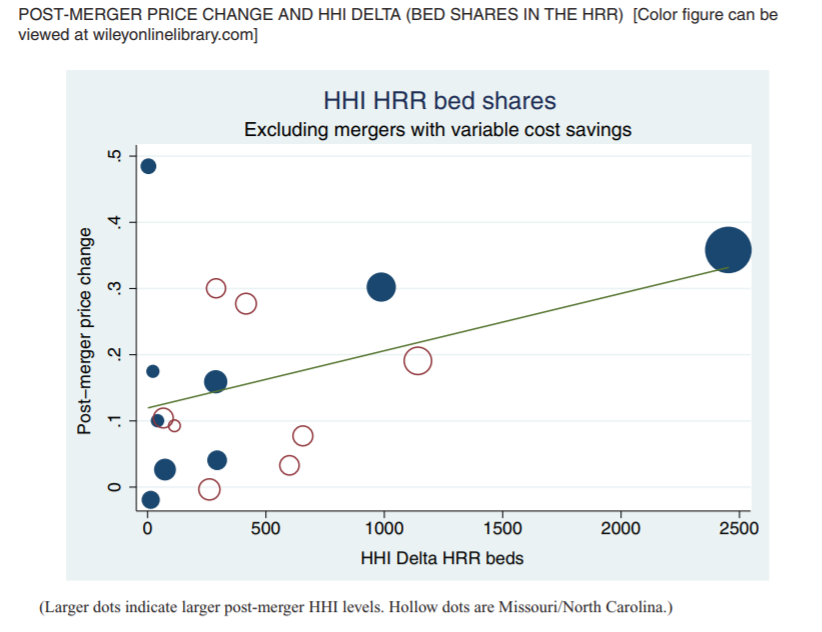
\includegraphics[width=\linewidth,height=\textheight,keepaspectratio]{hhi1.PNG} \\
    
\end{frame}
\begin{frame}
            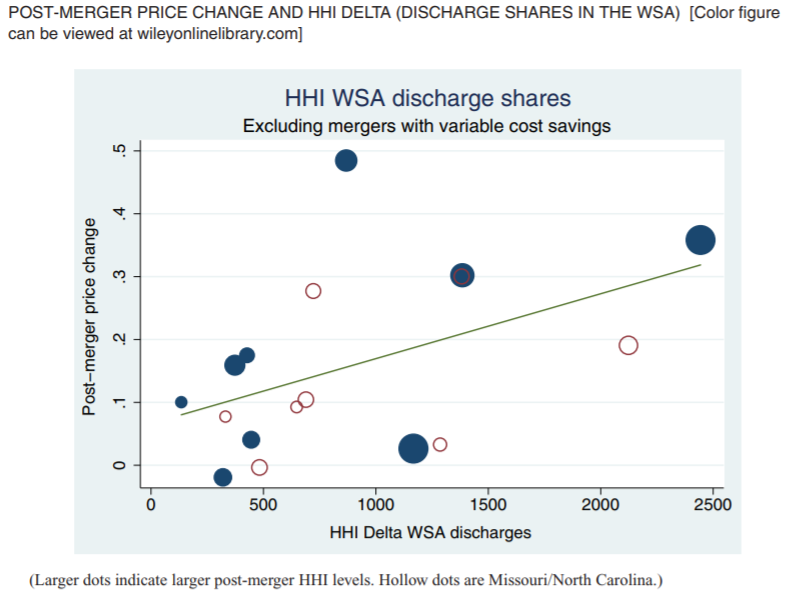
\includegraphics[width=\linewidth,height=\textheight,keepaspectratio]{hhi2.PNG} \\
    
\end{frame}
\begin{frame}
            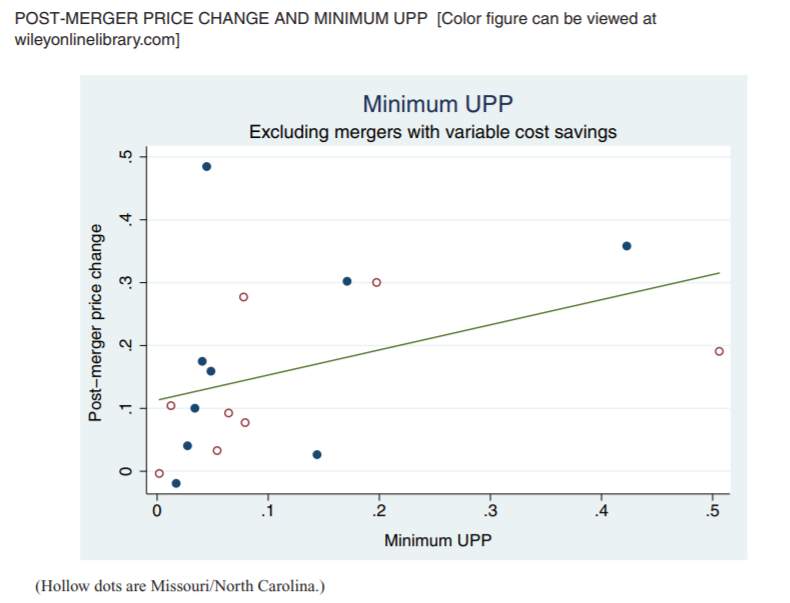
\includegraphics[width=\linewidth,height=\textheight,keepaspectratio]{upp.PNG} \\
    
\end{frame}
\begin{frame}
            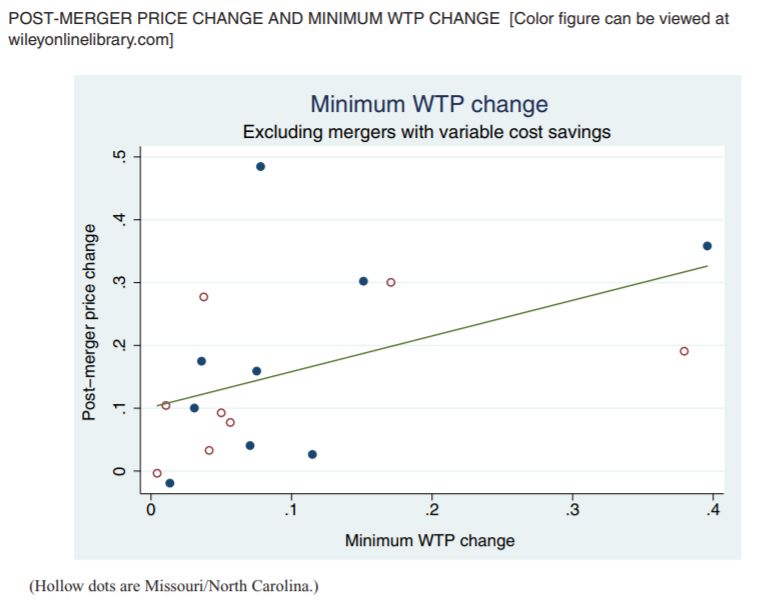
\includegraphics[width=\linewidth,height=\textheight,keepaspectratio]{wtp.PNG} \\
    
\end{frame}
\begin{frame}
            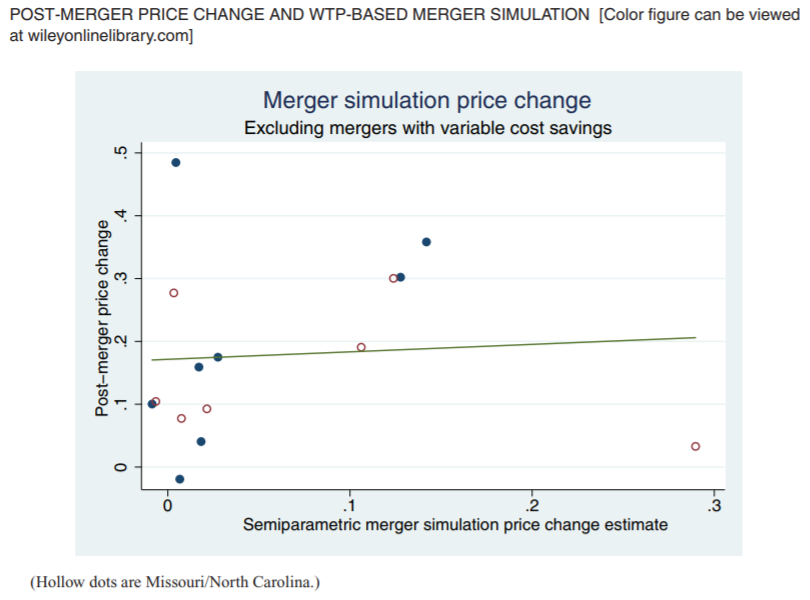
\includegraphics[width=\linewidth,height=\textheight,keepaspectratio]{msim.PNG} \\
    
\end{frame}
\begin{frame}{Takeaway and Limitations: Usual Disclaimers Apply}
\textbf{Takeaway:}  Willingness to Pay (WTP) and UPP outperformed performed HHI metrics in some circumstances. \\

\textbf{Limitations:}
    \begin{itemize}
        \item No statistically significant differences in full sample.
        \item This isn't a rigorous empirical test - there are a million things potentially wrong with the empirical specification.
        \item The question is whether the tests are even a reasonable first order screen.
        \item They are all useful if variable costs do not change, but how can we know if variable costs will change?
        
    \end{itemize}
\end{frame}

\end{document}
